\section{Methods}

\subsection{Model description}

The Ecosystem Demography version 2 (ED2) model simulates plot-level vegetation dynamics and biogeochemistry~\cite{Moorcroft_2001_ED,Medvigy_2009_ED2}.
By grouping individuals of similar size, structure, and composition together into cohorts, ED2 is capable of modeling patch-level competition in a computationally efficient manner.

Relevant to this work, ED2 includes a multi-layer canopy radiative transfer model that is a generalization of the two-stream solution of Sellers (1985). \nocite{SELLERS_1985_canopy}
In its default configuration, the ED2 radiative transfer model solves for the overall canopy albedo in two spectral ``bands''---visible and near-infrared---as a function of each cohort's leaf area index and PFT-specific parameters for leaf and wood reflectance and transmittance, canopy clumping factor, and leaf orientation factor.
The equations used are mostly adapted from the Community Land Model\cite{clm45_note}, but a summary of key features is as follows:

The direct radiation flux is modeled as an exponential attenuation curve through the canopy based on each layer's transmissivity ($\tau_r$),
which in turn is a function of the total area index ($TAI$) of the canopy layer and the inverse optical depth ($\mu_r$):

\begin{equation}\label{eq:tai}
  \tau_r = e ^ {- \frac{TAI}{\mu_r}}
\end{equation}

The total area index ($TAI$) is the sum of the wood area index ($WAI$) and the effective leaf area index, with the latter calculated as the product of the true leaf area index ($LAI$) and the clumping factor ($c$, defined on the interval $(0, 1)$ where 0 is a ``black hole'' (all leaf mass concentrated in a single point) and 1 is a homogenous closed canopy):

\begin{equation}
  TAI = c LAI + WAI
\end{equation}

The true leaf area index for each PFT is calcluated in two stages:
First, the total leaf biomass is calculated from the diameter at breast height via an exponential allometric equation parameterized for each PFT\@.
Second, the leaf biomass is converted to leaf area index through the PFT-specific specific leaf area (SLA).

The optical depth is calculated based on the projected area ($p$) and the solar zenith angle ($\theta$):

\begin{equation}
  \mu_r = \frac{\cos{\theta}}{p}
\end{equation}

The projected area ($p$) is a function of the leaf orientation factor ($f$):

\begin{equation}\label{eq:phi1}
  \phi_1 = 0.5 - f (0.633 + 0.33 f) \\
\end{equation}

\begin{equation}\label{eq:phi2}
  \phi_2 = 0.877 (1 - 2 \phi_1) \\
\end{equation}

\begin{equation}
  p = \phi_1 + \phi_2 \cos{\theta} 
\end{equation}

The diffuse radiation flux is more complicated because light is scattered internally within and between canopy layers.
Unlike the Community Land Model, which solves only for sunlit and shaded leaves,
EDR calculates the full canopy radiation profile by parameterizing the two-stream equations for each layer (as well as soil and atmosphere boundary conditions)
and then using a linear system solver to solve for the radiation profile.
For each layer, leaf and wood forward scattering ($\omega_+$) are just the sums of their respective reflectance ($r$) and transmittance ($t$) values:

\begin{equation}
   \omega_+ = r + t 
\end{equation}

Leaf and wood backscatter ($\omega_-$) are a function of their respective reflectance and transmittance values as well as the leaf orientation factor ($f$):

\begin{equation}
   \omega_- = \frac{r + t + 0.25 (r - t) {(1 + f)} ^ 2}{2 (r + t)} 
\end{equation}

Overall scatter ($\iota$) and backscatter ($\beta$) of all elements in a canopy layer is modeled as the average of leaf and wood scatter, weighted by their respective area indices:

\begin{equation}\label{eq:wl}
  w_l = \frac{LAI}{LAI + WAI}
\end{equation}

\begin{equation}\label{eq:ww}
  w_w = \frac{WAI}{LAI + WAI}
\end{equation}

\begin{equation}\label{eq:scatter}
  \iota = w_l \omega_{+,l} + w_w \omega_{+,w}
\end{equation}

\begin{equation}\label{eq:backscatter}
  \beta = w_l \omega_{-,l} + w_w \omega_{-,w}
\end{equation}

The inverse optical depth for diffuse radiation ($\mu_f$) is calculated from the coefficients $\phi_1$ and $\phi_2$ (see equations~\ref{eq:phi1} and~\ref{eq:phi2}):

\begin{equation}
   \mu_f = \frac{1 - \phi_1 \ln{(1 + \frac{\phi_2}{\phi_1 \phi_2})}}{\phi_2} 
\end{equation}

Note that $\mu_f$ simplifies to 1 when orientation factor is 0 (random, spherical distribution of leaf angles).
Collectively, these coefficients are used to calculate the optical depth for diffuse radiation ($\tau_f$):

\begin{equation}
  \epsilon = 1 - 2\beta
\end{equation}

\begin{equation}
  \lambda = \frac{\sqrt{(1 - \epsilon\iota) (1 - \iota)}}{\mu_f}
\end{equation}

\begin{equation}
  \tau_f = e ^ {\lambda TAI}
\end{equation}

The remaining coefficients are described in the Community Land Model manual~\cite{clm45_note}.
% Should probably finish this as an appendix or something at some point.

By default, ED takes as parameters PFT-specific leaf and wood reflectance and transmittance values with one value each for the visible and near-infrared spectral regions. 
For this analysis, I first modified ED to take an arbitrary number of leaf and wood reflectance transmittance values.
From there on, I simulated leaf reflectance and transmittance using the PROSPECT 5 leaf RTM (see Chapters 2 and 3).
For soil and wood reflectance, I used means of the corresponding spectra from Asner (1998), resampled to 1 nm resolution. \nocite{asner_1998_biophysical}
The final coupled PROSPECT-ED canopy radiative transfer model (hereafter known as ``EDR'') has 10 parameters for each PFT\@:
5 parameters for PROSPECT (number of mesophyll layers, and area-based chlorophyll, carotenoid, water, and dry matter contents),
specific leaf area,
base and exponent for the leaf allometry,
and clumping and orientation factors.

\subsection{Sensitivity analysis}

To provide a basis for understanding the behavior of EDR and how it compares to SAIL,
I performed a one-at-a-time sensitivity analysis to explore how EDR reflectance predictions vary with each parameter. 

Sensitivity of EDR to the PROSPECT parameters is effectively the same as sensitivity at the leaf level, kj

\subsection{Model calibration}

For model calibration, I selected 47 sites from the NASA Forest Functional Types (FFT) field campaign that contained plot-level inventory data (stem density, species identity, and DBH) coincident with observations of the NASA Airborne Visible/Infrared Imaging Spectrometer (AVIRIS).
These sites are mostly located in the United States Upper Midwest with several sites also in upstate New York and western Maryland, and include stands dominated by either evergreen or deciduous trees and spanning a wide range of structures, from dense groups of saplings (bottom right) to sparse groups of large trees (top left) (Figure~\ref{fig:sites}).
Based on ED's PFT definitions, these sites contained a total of five different temperate plant functional types: Early successional hardwood, northern mid-successional hardwood, late successional hardwood, northern pine, and late successional conifer.

\begin{figure}
  \centering
  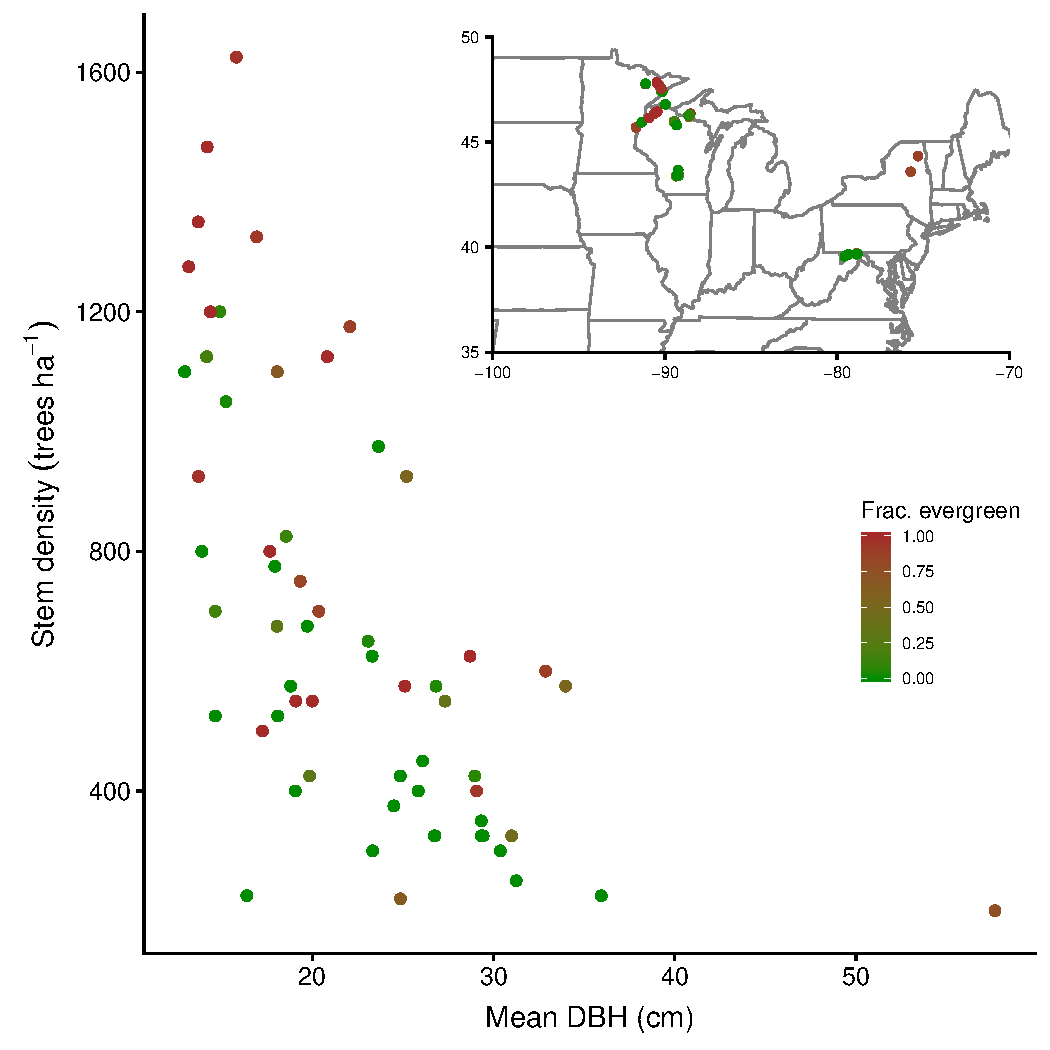
\includegraphics[width=\textwidth]{figures/sites_both.pdf}
  \caption{\
    Sites selected for analysis, in ``stand structure'' (\textit{main figure}) and geographic (\textit{inset}) space.
    Colors indicate the fraction of the stand that is made up of evergreen PFTs.
    Large points with labels indicate sites that were selected for forward simulations.
  }\label{fig:sites}
\end{figure}
% * <fer.istem@gmail.com> 2018-05-02T19:51:35.047Z:
% 
% not sure if it matters but the deciduousness gradient is not detectible from the color scheme, all points seem either 0 or 1 to me
% 
% ^.
% TODO: Change colors to be top cohort

I calibrated EDR using the same general Bayesian RTM inversion described in Chapter 3.
The inversion fit all sites simultaneously, such that at every MCMC iteration, the algorithm proposed a set of all parameter values for each PFT and simulated spectra for each site based on its observed composition and structure.
Because of unrealistic values in the shortwave infrared spectral region in the AVIRIS observations, likely caused by faulty atmospheric correction, I only calibrated the model with observations from 400 to 1300 nm.
% TODO: If I use it: Heteroskedastic variance model, fixed allometry parameter.
To generate the initial history state files required by EDR, I ran ED2 itself for one day in midsummer (July 1), starting from vegetation initial conditions based on observed composition and structure.

For priors on the five PROSPECT parameters and specific leaf area, I performed a hierarchical multivariate analysis (see Chapter 1) on PROSPECT parameters estimated from chapter 3 and, where available, direct measurements of specific leaf area. 
For priors on the leaf biomass allometry parameters, I fit a multivariate normal distribution to allometry coefficients from Jenkins et al.~(2003, 2004) using the \texttt{PEcAn.allometry} package. \nocite{jenkins_2003_allom,jenkins_2004_allom} 
For the clumping factor, I used a uniform prior across its full range (0 to 1), and for the leaf orientation factor, I used a weakly informative re-scaled beta distribution centered on 0.5.

I present posterior estimates for each parameter summarized as mean and 95\% confidence interval (Figure~\ref{fig:pda_posteriors}).
To evaluate the performance of the model, I compared the prior and posterior credible interval of the modeled spectra to the observations at each site (Figure~\ref{fig:sites}).
% * <dietze@bu.edu> 2018-05-02T22:08:48.140Z:
% 
% You shouldn't include links to analysis figures in the Methods section -- those should come in the Results
% 
% ^.
To assess any systematic errors in calibration, I also calculated the mean bias and root mean square error (RMSE) between the observed and mean predicted spectra binned across the visible (400--750 nm) and near infrared (750--1300 nm) spectral regions and plotted these values as a function of site mean DBH and stand density similarly to Figure~\ref{fig:sites} (Figure~\ref{fig:bias}).
As LAI in EDR is calculated from the parameters at each step, I also compared EDR estimates of LAI to observed values (Figure~\ref{fig:lai_validation}). %, and investigated the extent to which errors in predictions of spectra and LAI were related (Figure~\ref{fig:spec_lai}).

%\subsection{Forward simulation}

%I selected six sites for the ED2 forward simulation representative of the overall structure and composition space (Figure~\ref{fig:sites}). %TODO: Check this number. Drop SF03? Why don't I have it?
%Based on timber harvest data from the US Forest Service, I determined that one of these sites---OF05---was the site of a clear cut in 1982, which allowed me to simulate multidecadal dynamics of forest regrowth at this site by starting ED from near-bare ground in 1983.
%For the remaining sites, I performed shorter simulations starting from the earliest available survey data. % (2008 for XXX, 2009 for YYYY).
%I started all runs on June 2 of their respective start years (because ED runs are unstable when initialized from a leaf-off state), and stopped all runs on December 31, 2017.
%For meteorological drivers, I used the North American Regional Reanalysis~(NCEP 2005)\nocite{narr}, selected due to its high temporal (3 hour) and spatial (32 km) resolution, availability of all variables required by ED (such as temperature, precipitation, and downwelling short- and longwave radiation fluxes), and uninterrupted data availability across the simulation period (including up to one month before present).
%For soil inputs---namely, soil horizon classes and depths at each site---I extracted data from the US Department of Agriculture Soil Survey Geographic Database (SSURGO) using the \texttt{FedData} R package.

%For each site, I ran 50 ED2 ensemble members, sampling traits randomly from the joint posterior distributions estimated in the calibration step.
%Because the full vegetation dynamics version of ED2 is not configured to take PROSPECT spectra as an input, I set the parameters for leaf reflectance and transmittance to PROSPECT simulations averaged over the visible and near-infrared regions.
%When the ED2 simulations were finished, I ran EDR over the ED2 outputs, generating a daily time series of hyperspectral reflectance for each ensemble member and site.
%I then convolved these spectra to the six Landsat spectral bands using their known spectral response functions (as in Chapter 2),
%and compared the resulting spectral time series to observed Landsat time series for each site obtained using Google Earth Engine.
%To better capture the variability in the spectral data, I calculated the normalized difference vegetation index (NDVI) and tasseled cap spectral transformations (brightness, greenness, wetness) and used these as the basis for comparison.
